\documentclass[letterpaper,headings=standardclasses]{scrartcl}

\usepackage[margin=1in,includefoot]{geometry}
\usepackage{amssymb}
\usepackage{amsmath}
\usepackage{listings}
\usepackage{tikz}
\usepackage{float}

\DeclareMathOperator*{\argmax}{argmax}
\DeclareMathOperator*{\argmin}{argmin}

\usetikzlibrary{shapes,arrows}

\tikzset{
  block/.style    = {draw, thick, rectangle, minimum height = 3em, minimum width = 3em},
  sum/.style      = {draw, circle},
  input/.style    = {coordinate, circle},
  output/.style   = {coordinate, circle}
}

\lstset{basicstyle=\ttfamily,language=python,columns=flexible,breaklines=true,showstringspaces=false}

\title{Homework 5}
\subtitle{CS 559 - Neural Networks - Fall 2019}
\author{Matteo Corain 650088272}

\begin{document}

\maketitle

\section{Question 1}

\subsection{Data parsing and preprocessing}

Data have been parsed from the images and label files using a variation of the functions defined in the second homework for this purpose. Specifically:

In order to parse the images and labels files, two separate functions have been coded:

\begin{itemize}

    \item Function \texttt{idx\_images\_parse()} is used to parse the images files encoded in the IDX format; it performs the following actions:

        \begin{itemize}

        \item It opens the given file in \emph{read binary} mode;

        \item It reads the magic number using the \texttt{fromfile()} function provided by the Numpy library, which allows to read a certain number of elements (in this case, a single one) from a file given their data type (in this case, big endian \texttt{>}, unsigned integer \texttt{u} on four bytes \texttt{4}) and checks its correctness (it must be equal to 2051);

        \item In the same way, it reads the number of items and the dimensions of the input images into variables \texttt{n\_samples}, \texttt{n\_rows} and \texttt{n\_cols};

        \item Using the list comprehension syntax and the \texttt{fromfile()} function provided by the Numpy library, it reads \texttt{n\_samples} arrays of \texttt{n\_rows * n\_cols} elements stored as big endian, unsigned 8-bits integers (\texttt{>u1}), reshapes them to the correct format and stores them into the \texttt{samples} variable;

        \item It returns variables \texttt{n\_samples}, \texttt{n\_rows}, \texttt{n\_cols} and \texttt{samples}.

        \end{itemize}

    \item Function \texttt{idx\_labels\_parse()} is used to parse the labels files encoded in the IDX format; it performs similar actions with respect to the previous one, the only differences being that in this case samples dimensions are not present and that data items are represented by single 8-bits elements.

\end{itemize}

With respect to the functions used for the second homework, some preprocessing is done on the data before feeding them to the network as training samples. In particular, the following preprocessing has been applied:

\begin{itemize}

    \item Input pixel values have been normalized to 1, by dividing each component by 255 (they are stored as 8-bits unsigned integers);
    
    \item Labels have been mapped on their binary vector representation, using the \texttt{label\_to\_array()} function from homework 2.

\end{itemize}

Scaling the inputs allows for avoiding the need of training large weights for the network, while label mapping is useful since it is not necessary to reconstruct the binary representation each time it is needed (it is computationally easier to extract the argmax, when necessary).

\subsection{Network construction and training}

In order to properly represent the different networks, a \texttt{Network} class has been defined. Its constructor takes as arguments three lists, the first one containing the initial weights matrices (biases included) of each layer of the network, the second containing the function pointers corresponding to the activation functions of each layer of the network and the third the function pointers of the derivatives thereof. The class presents the following methods:

\begin{itemize}

    \item \texttt{feedforward()}: it feeds the network with the input $x = y_0$, computing for each layer the corresponding value of the local field $v$ and of the output $y$:
    
    $$ v_i = W_i \left[ \begin{matrix} 1 \\ y_{i - 1} \end{matrix} \right] $$
    $$ y_i = \phi_i(v_i) $$
    
    \item \texttt{backpropagate()}: it estimates the value of the gradient of the energy function $\nabla E$ through the backpropagation algorithm, for an input pattern $x$ with desired output $d$; this is performed in three steps:
    
    \begin{itemize}

        \item In the first step, the $v$ and $y$ vectors of the induced fields and outputs of each neuron are computed through the \texttt{feedforward()} method;

        \item In the second step, the delta signals are calculated, in reverse order of $i$:
        
        $$ \delta_L = (d - y_L) \cdot \phi'_L(v_L) $$
        $$ \delta_i = \underline{W_{i + 1}^T} \delta_{i + 1} \cdot \phi'_i(v_i), i = L - 1, \dots, 1 $$

        Where the underline denotes the weight matrix in which the first row (the one related to the bias term) has been removed.

        \item In the third step, delta signals are used to compute the effective components of the desired gradient:
        
        $$ \frac{\partial E}{\partial W_i} = -\delta_i \left[ \begin{matrix} 1 \\ y_{i - 1} \end{matrix} \right] $$

    \end{itemize}
    
    \item \texttt{errfunc()}: it calculates the value of the error function for the entire training set, averaging the squared value of the norm of the difference between the desired outputs and the effective outputs (computed through the \texttt{feedforward()} method):
    
    $$ E = \frac{1}{|\mathcal{S}|} \sum_{i = 1}^{|\mathcal{S}|} || d_i - y_{i,L} ||^2 $$
    
    \item \texttt{test()}: it calculates the accuracy of the network on the test set, by summing a value of 1 each time the classification is correct (that is, $ \argmax{y_{i,L}} = \argmax{d_i} $) and dividing by the number of test samples:
    
    $$ a = \frac{1}{|\mathcal{T}|} \sum_{i = 1}^{|\mathcal{T}|} \alpha_i, \; \alpha_i = \begin{cases} 1 & \text{if } \argmax{y_{i,L}} = \argmax{d_i} \\ 0 & \text{otherwise} \end{cases} $$
    
    \item \texttt{train()}: it performs a gradient descent, backpropagation-based training of the network; it takes as parameters:
    
    \begin{itemize}

        \item The training samples and labels;
        \item The test samples and labels (to record the test set accuracy for increasing epochs);
        \item The initial learning rate $\eta$;
        \item The target value of the error function $\epsilon$;
        \item The batch size for the learning procedure;
        \item A string suffix to be used for storing computed quantities in appropriate files for later usage (e.g. plotting) without having to fully recompute them.
    
    \end{itemize}

    The procedure performs the following actions:

    \begin{itemize}
        
        \item It initializes the \texttt{errors} and \texttt{tests} lists with the initial values of the error function and of the test set accuracy;
        
        \item It enters the training loop, whose stopping conditions are expressed on the number of epochs (it has to be lower than the configured limit) and on the value of the error function (it has to be greater than the configured limit);
        
        \item It loops on the training samples, computing for each of them the value of $\nabla E$ through the \texttt{backpropagate()} method, then updates the weight matrices of the different layers using the standard gradient descent rule;
        
        \item It registers the value of the error function and the accuracy on the test set for the current weights;
        
        \item If the value of the error function increases among two consecutive epochs, it reduces the learning rate of a factor of 0.9.
        
        \item When the training loop is computed, the final weights and the lists of errors and accuracy values are saved to file and returned.

    \end{itemize}

\end{itemize}

All the described operations have been implemented using the opportune functions and operators provided by the Python language and the NumPy library.

\subsection{Tested networks and results}

For the sake of the exercise, three networks have been tested, whose main parameters are presented in table \ref{net_params}.

\begin{table}[h]
    \centering
    \begin{tabular}{|c|c|c|c|c|c|c|c|c|c|c|}
    \hline
    Network \# & Layers & $n_1$ & $n_2$ & $n_3$ & $\phi_1$ & $\phi_2$ & $\phi_3$ & $\eta$ & $\epsilon$ & Epoch limit \\ \hline
    1 & 2 & 100 & 10 & - & tanh & sigmoid & - & 0.01 & 0.01 & 5000 \\ \hline
    2 & 2 & 200 & 10 & - & tanh & sigmoid & - & 0.01 & 0.01 & 5000 \\ \hline
    3 & 3 & 100 & 100 & 10 & tanh & tanh & sigmoid & 0.01 & 0.01 & 5000 \\ \hline
    \end{tabular}
    \caption{Parameters of the tested networks}
    \label{net_params}
\end{table}

In all three cases, the weight matrices have been initialized using random values drawn from a normal distribution with $\mu = 0$ and $\sigma = m^{-1}$, where $m$ represents the number of inputs of each specific layer.

For the first network, it has been chosen to use two layers since it is proven that any two-layer network is able to approximate any given function with arbitrary precision; the choice of the number of neurons in the hidden layer has been dictated by the necessity of keeping the computational cost of the training procedure within an acceptable range. The choice of the sigmoid activation function for the output layer has been driven by the fact that its output range is entirely positive (it does not make sense, in this context, to have negative output values).

Once the first network was trained and tested, the other two networks were considered for comparison as variations of the first having a total of 100 additional neurons, respectively in a single and in two hidden layers. Results of the training process are shown in table \ref{net_results}.

\begin{table}[h]
    \centering
    \begin{tabular}{|c|c|c|}
    \hline
    Network \# & Epochs to convergence & Test set accuracy \\ \hline
    1 & 67 & 97.64\% \\ \hline
    2 & 44 & 97.90\% \\ \hline
    3 & 26 & 97.84\% \\ \hline
    \end{tabular}
    \caption{Training results for the tested networks}
    \label{net_results}
\end{table}

As it can be seen, the three networks have very similar performance when evaluated on the test set, but they substantially differ in their training performance. As it could be expected, the network requiring the most epochs to train was the first one, due to the more limited number of neurons it contains. Increasing the number of neurons in a single hidden layer presents some improvements (the number of epochs to convergence decreases), although this is only a theoretical improvement since the actual time needed to train such a network is considerably longer than in the previous case (matrix multiplication has is a problem with more than quadratic complexity in the dimensions of the matrices). The overall best network, both in terms of epochs to convergence and effective training time, is the 3-layer one, showing as expected more abstraction capabilities of the others.

Figures \ref{errors_plot} and \ref{tests_plot} show respectively the value of the error function and the test set accuracy for increasing number of epochs for the three networks (epoch 0 is excluded because significantly out-of-scale). It is possible to notice how the performances of network 3 are consistently better than the ones of network 2, which in turn has better performances than network 1, throughout the entire learning process.

\begin{figure}[H]
    \centering
    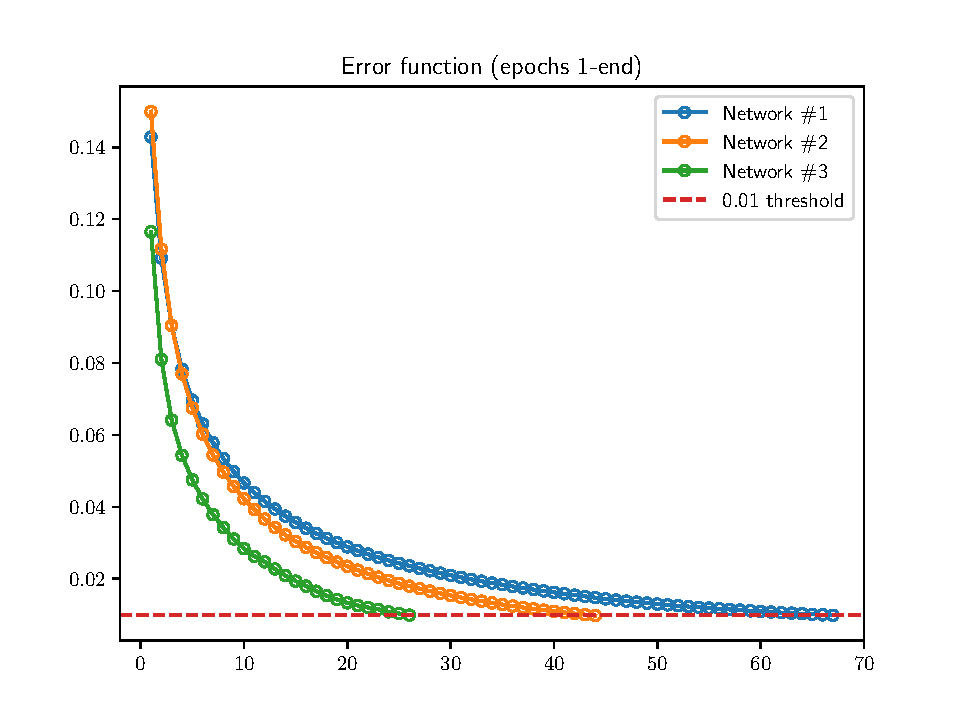
\includegraphics[width=.7\linewidth]{errors.pdf}
    \caption{Error function for increasing number of epochs}
    \label{errors_plot}
\end{figure}

\begin{figure}[H]
    \centering
    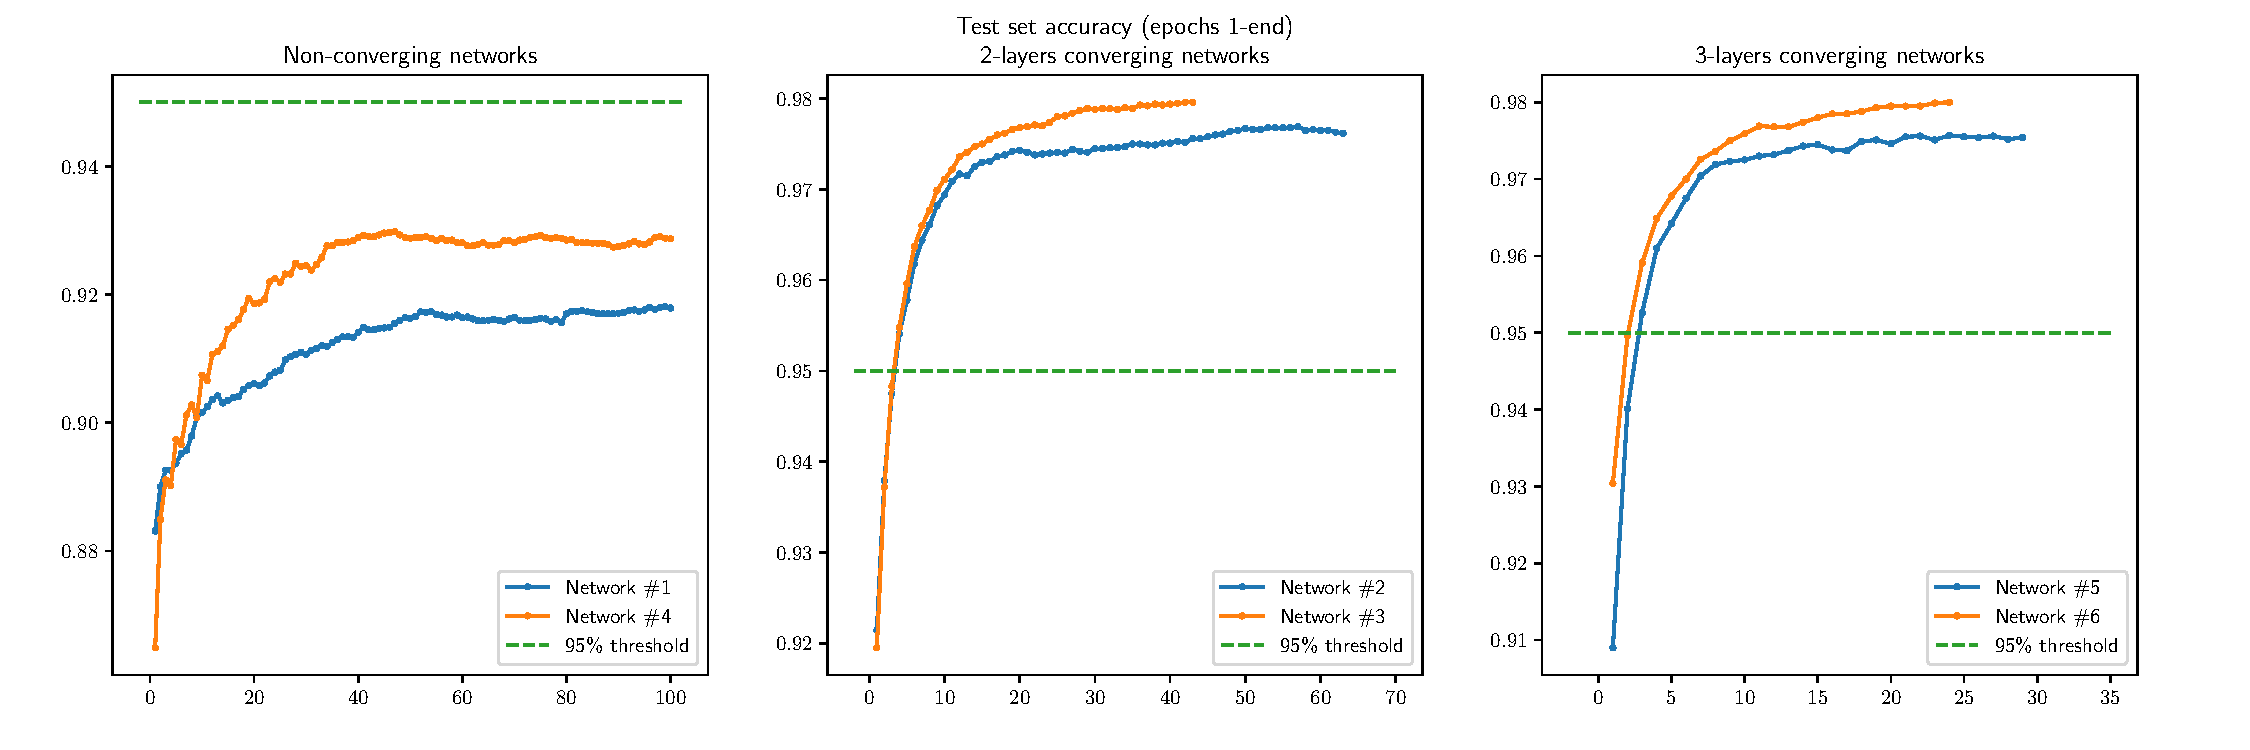
\includegraphics[width=.7\linewidth]{tests.pdf}
    \caption{Test set accuracy for increasing number of epochs}
    \label{tests_plot}
\end{figure}

\subsection{Complete Python code}

\subsubsection{Data parsing functions}

\lstinputlisting[basicstyle=\ttfamily\scriptsize]{idxfuncs.py}

\subsubsection{Network class definition}

\lstinputlisting[basicstyle=\ttfamily\scriptsize]{network.py}

\subsubsection{Training of network 1}

\lstinputlisting[basicstyle=\ttfamily\scriptsize]{net1.py}

\subsubsection{Training of network 2}

\lstinputlisting[basicstyle=\ttfamily\scriptsize]{net2.py}

\subsubsection{Training of network 3}

\lstinputlisting[basicstyle=\ttfamily\scriptsize]{net3.py}

\end{document}